\TOWRITE{ALL}{Proofread WP 1 Management pass 1}
\begin{draft}
\TOWRITE{PS (Work Package Lead)}{For WP leaders, please check the following (remove items
once completed)}
\begin{verbatim}
- [ ] have all the tasks in this Work Package a lead institution?
- [ ] have all deliverables in the WP a lead institution?
- [ ] do all tasks list all sites involved in them?
- [ ] does the table of sites and their PM efforts match lists of sites for each task?
      (each site from the table is listed in all relevant tasks, and no site is listed
      only in the table or only at some task)
\end{verbatim}
\end{draft}

\begin{workpackage}[id=applications,wphases=0-48,swsites,
  title=Applications and demonstrations,
  short=Applications,
  lead=XFEL,
  % EGIRM=4,
  CDSRM=12,
  INSERMRM=24,
  QSRM=6,
  % SILRM=4,
  SRLRM=9,
  UIORM=12,
  UPSUDRM=4,
  WTTRM=3,
  XFELRM=36,
  EPRM=4,
]
\begin{wpobjectives}
  The objectives of this work package are
 \begin{compactitem}
   \item to guide the development of core tools by simultaneously
     developing and using applications in diverse fields with active
     scientists from these fields, and
   \item demonstrate that the tools we develop are valuable to diverse
     fields of science, thus ensuring we develop e-infrastructure and
     services which can cater for a broad customer base of EOSC.
 \end{compactitem}
\end{wpobjectives}

\begin{wpdescription}

  In order to ensure that the work we do is beneficial to science and
  society, we will develop applications in diverse domains, using the
  components developed in work packages \WPref{core} and
  \WPref{ecosystem}.

  By developing applications simultaneously with the core
  infrastructure and services, we ensure that we are serving
  real-world use cases with our development.  Feedback from
  applications development can guide development of core features.  In
  addition to helping ensure that our work is useful to the chosen
  application domains, the applications serve as demonstrations of
  this utility.

  One of the key aspects of Jupyter that make it the choice for
  \TheProject, is that it is generic, based on open protocols and
  widely useful in diverse domains, from physics to life sciences to
  education and the global community working with public and private
  data. We have selected a number of applications in a variety of domains
  to demonstrate the broad impact of \TheProject.

\end{wpdescription}

\begin{tasklist}
% add tasks from task directory here
% % template for a task
% each task should be added to exactly one workpackage
% in the workpackage task list
\begin{task}[title=Task title,
  id=task-id,
  lead=XXX,
  PM=1,
  wphases={0-48},
  partners={XXX,SRL}
]
  The task includes the following activities
  \begin{compactitem}
  \item ...
    (\delivref{workpackage}{deliv-id})
  \end{compactitem}
\end{task}

\begin{task}[
  title=Teaching with Jupyter technology,
  id=teaching,
  lead=EP,
  PM=8, % EP: 4PM, UPSUD: 4PM
  wphases={0-48},
  partners={EP,UPSUD}
  ]

  The Mathematics department at Ecole polytechnique as well as ... at UPSUD..
  {\bf preciser} have started a reform of their various teaching offer based on
  Jupyter for two years and several courses of the Bachelor program, 2nd and 3rd
  year of Engineering school and Master program have already begun relying on a
  strong use of Jupyter notebooks / JupyterHub\footnote{MAP551 - 2nd yer course
  MAP411 - AMS X02 - Mooc INRIA preciser?} and this will continue with a strong
  support of the Dean of undergraduate studies and of graduate studies. Besides
  several software and research engineers in applied mathematics have been
  recruited and participate in this effort, as well as a administration engineer
  in order to help in terms of building an infrastructure dedicated to Jupyter
  with the support of the head of the Ecole polytechnique in order to diffuse
  the effort into various other departments (Physics, Mechanical Engineering,
  Biology...), where already some courses are starting based in Jupyter. The
  link with the computer science club of students of Ecole polytechnique (Binet
  Reeau) has also been created with the project and a community is emerging.

  This framework is ideal for the project for two reasons : 1- it offers both
  the test infrastructure and community, and some identified courses and
  Professor / Engineers / Students, who will test the newly designed tools
  (nbgrader / novel JupyterHub technology) and provide some feedback in order to
  improve them (this can be conducted within the timing of the project since the
  framework is already present), 2- It creates a reactive community of students
  and researchers within Ecole polytechnique and Paris-Sud, where the
  dissemination of the project tools and experience will be easy, which will
  organize Jupyter days on a regular basis, where the demonstrators of the
  project for tasks XXX will be presented and discussed. {\bf link with WP
  dissemination}

  The task includes the following activities
  \begin{compactitem}
  \item Reinforcement of the use of Jupyter technology in Courses at all the level of Maths and Data Science at Ecole polytechnique and Psud...,
  \item Test of the new developments and feed back to tasks ... (List of courses? Link Data science - JB?)
  \item Organization of a Jupyter day\footnote{In 2018 \url{http://www.cmap.polytechnique.fr/~massot/Personal_web_page_of_Marc_Massot/JupyterX.html}} every year with demonstration of Jupyter new tools
    (\localdelivref{deliv-id})
  \end{compactitem}
\end{task}

% template for a task
% each task should be added to exactly one workpackage
% in the workpackage task list
\begin{task}[
  title=Reproducible X-ray crystallography workflows at European XFEL,
  id=reproducibility-xfel,
  lead=XFEL,
  PM=36,
  wphases={6-48},
  partners={XFEL}
  ]

\emph{Summary:}

  European XFEL is a research facility that provides X-ray Free
  Electron Laser (XFEL) light to image structures at the nanoscale. It
  is currently the world's most brilliant laser, created in a 3.4km
  long tunnel, and supporting user experiments since September
  2017. These imaging capabilities from European XFEL and similar
  services from synchrotron and neutron sources, underpin lots of
  fundamental and applied research, in domains ranging from fundamental
  physics and material science to biochemistry and drug design.

  All of the data recorded at European XFEL will be made freely
  available after an embargo period of three years
  \cite{EuXFEL-datapolicy-2017}. This provides scientific transparency
  and is expected to enable better exploitation of the data, as more
  researchers than those conducting the experiments have access to the
  results. If the analysis steps are not carefully recorded, there is a risk
  that the necessary understanding of the data is lost by the time it
  is made public or subsequently, greatly reducing its scientific
  value.

  We are keen to complement this open data access to the actual data
  with open access to reproducible data analysis, to confirm
  conclusions drawn and to significantly lower the barriers for
  re-analysis with new tools or for new research purposes.

  A task in the EC funded project Photon and Neutron Open Science
  Cloud (PaNOSC) is using the Jupyter Ecosystem tools as they are in
  2019 to provide interactive data analysis services to complement the
  data: through use of Jupyter Notebook and exploitation of the
  mybinder.org service, this activity will reduce the barrier for
  interactively exploring the data, understanding and making use of
  the data, and to do this through a central portal such as EOSC.

  Here, we combine and use the new developments of this
  proposal to enable new qualities of open science services, and to
  demonstrate the potential impact of these improvements for a wide
  set of EOSC services through a demonstrator in Photon Science.

  \medskip \emph{Context}: The very first experiments at European XFEL
  produced as little as 45 terabytes of data on average, but as the
  facility develops, the amount of data produced per time is expected
  to grow substantially: Given the rate of light pulses, there is the
  potential to produce up to a petabyte of data within the beam time
  of one experiment (typically one week). These significant amounts of
  data need to be complemented by complicated workflows to convert the
  data into insight through data analysis. Derived results of such
  data analysis are typically much smaller in size and useful to
  archive together with the raw data. To explain how they have been
  obtained, the particular workflow of data analysis also needs to be
  archived.

  \medskip \emph{Vision}: At European XFEL we will use Jupyter notebooks to facilitate
  this workflow: the simplest model would be to use one notebook per
  workflow. Once the data capture from the experiment is completed,
  this notebook can be executed (without being displayed in a web
  browser) to start processing the data. When the notebook has
  completed execution, it is saved, and contains the analysis results
  (it may of course also created files on disk as part of the
  process).

  A particularly useful aspect of the notebooks is that they mix data
  analysis commands with outputs, and that the notebook provides a
  complete (and thus reproducible) summary of the data analysis when
  it succeeds with the execution. Should the execution fail, for
  example half-way through the notebook, then derived results obtained
  prior to the error occurring are preserved and can be inspected. The
  error is embedded in the notebook and appears after the command that
  has triggered the error; which helps with debugging the process.

  This is of particular interest as the data analysis processes at
  European XFEL may fail not because of software errors but due to
  variation in the data that require (manual) expert adjustments of
  parameters. The ``failure'' of such an analysis workflow
  (represented through the Notebook) is thus not exceptional, but a
  common occurrence. The scientist conducting the experiment is
  sufficiently skilled to modify the parameters and wants to either
  re-execute the notebook from the beginning or to continue from the
  point of failure. The notebook caters for both use cases. The
  modified notebook would need to be preserved of course to provide
  reproducibility of the derived results that the notebook has
  computed.

  We are aiming for re-executability of the notebook for the lifetime
  of the data. The life time of the archived data at European XFEL is
  currently guaranteed for 5 years and aimed to be 10 years
  \cite{EuXFEL-datapolicy-2017}. It is possible though, that data used
  for publications will be preserved for longer, and it would be
  highly desirable to keep the data analysis re-executable for the
  same period of time, potentially well exceeding 10 years.

  \medskip \emph{This task} includes the following activities:
  \begin{compactitem}
  \item Use the software archive for reproducible computation
    (as co-developed in \taskref{ecosystem}{reproducibility}), with
    the aim to provide reproducible computation environments for data analysis at
    European XFEL that remains executable for the same duration as the
    data is kept (currently aiming at 10+ years, at least 5 years).

    As is common in computational science, software used at XFEL often
    relies on specific combinations of libraries, often with
    particular version requirements. Thus we will need a dedicated
    software archive that holds all relevant packages and source codes
    that are required to build the required computational environments
    (see \taskref{ecosystem}{reproducibility}) to ensure they are
    available even if an open source software provider decides to
    remove their repositories, or changes the API of a package, or
    Github decides to terminate their business.

    Applying the work from \taskref{ecosystem}{reproducibility} in the
    context of a production system will demonstrate its true utility,
    and provide important feedback for the design. There will be
    iterative feedback and refinement of the service.

  \item Extend the use of notebooks from \emph{interactive} data
    exploration and analysis at European XFEL to also provide
    computational work flows via (semi-)automatic execution of
    notebooks as described above. The work done in
    \taskref{core}{collaboration} will allow us to execute notebooks in
    the background, and to connect to the running notebook process to
    display or inspect progress, or to modify a notebook if the
    science requires it.

    By doing so, we can make the standard analysis that is carried out
    by the facility available on EOSC as a service. By using one tool
    (the notebook) we simplify process for users and for the research
    facility.

  \item Work with partners in the PaNOSC project to evaluate and use
    these advances for other Photon and Neutron Science research
    facilities.

  \item Evaluate the chosen workflow design and experience from using
    it in a real-world context; make this available as a report and
    through presentations/workshops to interested organisations and
    facilities. (Deliverable \localdelivref{xfel-workflows})
  \end{compactitem}

  \TODO{Mention PaNOSC -- add project REFERENCE}
  \TODO{Mention widgets for interactive work?}
  \TODO{Make link to EOSC more obvious}
  \end{task}

\begin{task}[
  title=Astronomy application,
  id=astro,
  lead=CDS,
  PM=18,
  wphases={0-48},
  partners={CDS,QS,WTT,SRL}
]

  Context: The Strasbourg Astronomical Data Center (CDS) is scientific data 
  center hosted by the Observatory of Strasbourg. The CDS plays a unique and 
  essential role in astronomy by adding value to published and reference data. 
  CDS runs astronomical services that
  provide data for the world-wide astronomy research community. Its three main
  services (SIMBAD, VizieR and Aladin) are heavily used with up to one million
  queries per day.  These services be accessed through web interfaces, mainly
  for human interaction, as well as through programmatic interfaces, including
  the standardized protocols defined by the International Virtual Observatory
  Alliance.

  Python and notebooks are rapidly increasing in importance for astronomy 
  research. Indeed, Python for Astronomy software ecosystem has known a 
  constant steady growth in the latest years, as shown in 
  figure~\ref{fig:python-astro-citations}.


  We will develop a Jupyter-based framework to efficiently access, explore,
  visualize and analyze reference data that are available through CDS services 
  as a real example of using open astronomy data.
  We will provide scientific users with a set of customizable Jupyter notebooks
  for visualization and analysis tasks, providing a new level of
  interoperability with python libraries and notebooks as is highly demanded
  by the astronomy research community.

  The focus is on the two following user stories:
    \begin{compactitem}
        \item analysis of catalogue data results, up to billions of rows.
              Tabular data is the typical output of SIMBAD and VizieR data.
        \item modular dashboard-like interface providing a top level
              interactive view of the available data for a given astronomical
              object and enabling loading and analysis of those data.
    \end{compactitem}


  This task will build on existing Python libraries to access CDS data
  (\textit{astroquery.[cds/simbad/vizier/xmatch]}). For visualization, we will 
  use proven tools like \textit{GLUE} and \textit{ipyvolume}, which are now 
  built upon the Jupyter stack.
  We will also make significant improvement to existing Jupyter widgets 
  (\textit{ipyaladin}, interactive sky atlas running in the notebook) and 
  develop a new widget to offer a tree-like view of available datasets.

  We will also develop Python libraries to allow integration and usage in
  notebook of existing CDS infrastructure services, namely CDSLogin (which
  provides authentication) and CDS MyData (remote storage space for tabular
  data).
  This will allow the user to interact with one's personal storage space from
  the notebook. It will also allow for advanced customisation of the interface 
  to fit user needs.

  The work is organised with a 2 stage approach. Firstly, the generated 
  notebooks will run locally on user machines (milestone). Following the 
  Binder development in \WPref{eosc}, we will aim to run these notebooks 
  on the European Binder service. The deliverable of this task will be a 
  demonstrator available to the scientific user community 
  (\localdelivref{application-astro}).
\TODO{This two stage approach (above and below) is good. Can we split
  this into two tasks, or link each to a different milestone, to make
  this more visible?}
\COMMENT{\blue{Agreed to have a milestone. How should that be described?}}


  Access to the notebooks will be provided as a one-click action option from
  SIMBAD and VizieR results pages.
  Thus, providing with a one-click way of visualizing, filtering and analyzing
these potentially large tables will bridge the gap between access and analysis
of the data, with zero installation for the user.
  For specific science cases, we will explore rendering of notebooks with 
  interactive widgets through "Voila", as to allow users not familiar with 
  Python to benefit from the Jupyter notebook framework.

  These new developments will be highly visible to the large number of astronomers who use the CDS services (50,000 unique visitors per month) and such tools are in high demand by these users.

  The CDS expertise in astronomy data and interfaces will be profitably combined with expertise of BOSSEE partners to ensure the deployment of high quality widgets (Simula, WildTree Tech, QuantStack).

\begin{figure}[ht]\centering
  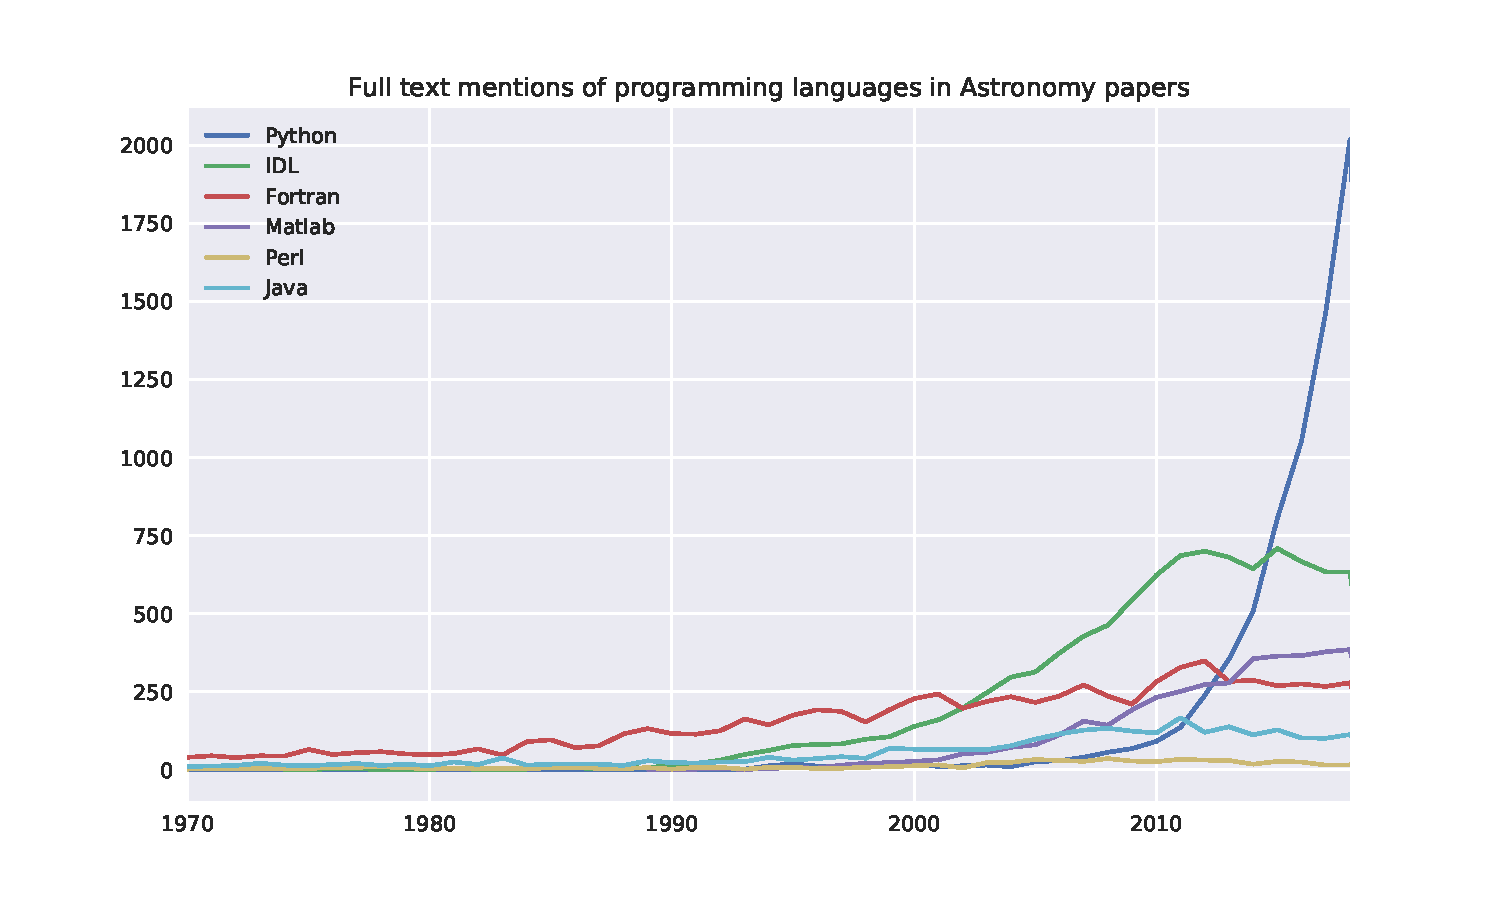
\includegraphics[width=0.8\textwidth]{python-astro-citations}
  \caption{Mentions of programming languages in refereed Astronomy papers, extracted from ADS. Python usage has increased dramatically in the recent years.}\label{fig:python-astro-citations}
\end{figure}

Deliverable: \localdelivref{application-astro}


\end{task}

\begin{task}[
  title=Geosciences application,
  id=geoscience,
  lead=UIO,
  PM=24,
  wphases={0-48},
  partners={QS,SRL}
]

% Scientific description

The amount of geospatial data from a variety of sources, including satellite observations, 4D simulations and in-situ observations, contributed by volunteers
or state agencies keeps increasing. In many disciplines, managing this large volume
has become a challenge, and the old approach of downloading datasets for a local
analysis has become intractable.

The heterogeneity of the tools used in different institutions to deal with
large geographical datasets makes it difficult for researchers to share the outcome
of their work in a reproducible fashion.

In this context, Jupyter is now emerging as a standard exploration tool for
geospatial analysis, climate science, geology and by data providers in these areas.

To mention a few,

\begin{itemize}
\item
   the \emph{PanGeo} platform (Funded by the NSF, NASA, and the Alfred P.
   Sloan Foundation) is built upon Jupyter, JupyterHub, Binder, and Dask.
\item
   the \emph{Joint Research Centre Earth Observation Data and Processing Platform}
   (JEODPP) relies on Jupyter, JupyterHub and ipyleaflet as its main user
   interface.
\item
   the \emph{google earth engine} platform also offers a jupyter-based user
   interface allowing the visual exploration of the data with ipyleaflet.
\end{itemize}

In these three cases, deferred processing is used to restrict computation to
the extent of the area displayed in the map viewer, which allowed these
platforms to scale up to petabytes of data. In all examples, interactive
visualization is a key feature of the platform. Beyond tile-based
2-D visualization, the ability to efficiently process and visualize vector
or 3-D data is also becoming critical.

The BOSSEE team, which comprises the main authors of the technologies upon
which these platforms are built (Jupyter, JupyterHub, Binder, ipyleaflet),
together with the Department of Geosciences of the University of Oslo, are
in a unique position to bring these technologies together in the context of
EOSC.

This demonstrator will focus on tools for two transversal research projects

\begin{itemize}
\item LATICE (Land-Atmosphere Interactions in Cold Environments)
\item EarthFlows (Interface Dynamics in Geophysical Flows)
\end{itemize}

The work items for this demonstrator fall in two main categories:
visualization and geographical data processing tools.

\textbf{Visualization}

\begin{compactitem}
  \item Improvement upon existing mapping tools for specialized
    visualization of in-situ and model-generated data arizing in
    specific use cases (Land, river-runoff, ocean, ice, wave and
    atmosphere models, particle dispersion models, oil spill models,
    etc.).

    This may take the form of additions to the \emph{ipyleaflet} and
    \emph{folium} extentions to JupyterLab, as well as the production of
    curated examples in the documentation of ipyleaflet addressing these
    specific use cases.

  \item Improvements of the tooling for 3-D visualization of
    geographical datasets in the Jupyter notebook, for use cases such as
    displaying volcanic plumes (injection of aerosols in the various
    atmospheric layers), the quasi biennial oscillation (inversion of
    the wind direction in the tropical stratosphere), atmospheric rivers
    (flowing column of condensed water vapour in the atmosphere) and
    also at smaller scales to visualize 3-D discrete particle simulations
    of sheared granular fault zones.
\end{compactitem}

\textbf{Collaboration with Jupyter with specialized tools for earth sciences}

\begin{compactitem}
  \item adding the ability to interactively integrate information or corrections
    observed during field trips, correspdonding to specific geographical locations.

    \TODO{Concurrent editing links to real-time editing from the
    core WP2 - mention link?}

  \item adding the ability to deploy Jupyter-based applications together with
    the correspdonding execution environment, both in the form of a runnable
    notebook with \emph{Binder} or as a read-only yet interactive \emph{Voila}
    dashboard.
\end{compactitem}

\textbf{Teaching geo-sciences with Jupyter}

  All these developments will be used both for scientific research and
  in the classroom for teaching master's students with best practices
  in open science.

  The Geosciences use case will make it possible to demonstrate the
  effectiveness of the BOSSEE co-design approach. The main challenges
  will be on the one hand to learn to take advantage of feedback given
  by users (either novices or experts) and on the other hand for
  BOSSEE developers to adapt their communication and language as well
  as their offer to the Geoscience. This will lead the way for
  on-boarding new communities.

  \TODO{The transversal research plays into the desired ``services that
    encourate collaborative interdisciplinary work'' that are desired
    by this call; this is good. Can you imagine that some of these
    facilities can be used via the EOSC? That would be a good
    addition. For example, one could use the BinderHub installation
    that we expect on the EOSC. }


\end{task}

\begin{task}[
  title=Nuclear Medicine application,
  id=opendose-analysis,
  lead=INSERM,
  PM=24,
  wphases={0-24},
  partners={}
]
  % Scientific description
  Nuclear Medicine is a field of medicine where radioactive material
  (radiopharmaceutical) is used for diagnostic and therapy. Even though the
  majority of Nuclear Medicine procedures (90\% according to successive EANM
  surveys) are diagnostic examinations, therapeutic applications tend to
  develop and drag more and more attention, for example for the treatment of
  neuroendocrine tumours \cite{Bodei2009}.

  The formalism used to objectively characterise the irradiation process is
  similar for both application types: it was introduced in the late 60s by the
  MIRD (Medical Internal Radiation Dose) committee of the American Society of
  Nuclear Medicine (SNM). This formalism \cite{loevinger1991mird} requires two
  independent quantities; the radioisotope cumulated activity ($Bq.s$) in the
  source (tissue/organ) and the mean absorbed dose to a given target
  (tissue/organ) per radioisotope disintegration (S-value,
  $Gy.Bq^{-1}.s^{-1}$). The S-value calculation requires a clear definition of
  the geometry of the patient (or the model) and radioisotope decay
  characteristics, it can be expressed as a linear combination of
  yields/energies ($J$) and Specific Absorbed Fractions (SAF, $g^{-1}$).

  The calculation of SAFs involves radiation transport modelling and energy
  deposition scoring in anthropomorphic models, usually based on Monte Carlo
  simulation. Historically, SAFs were computed from mathematical models -
  simplistic approximations to human geometry. The advent of voxel-based
  computational models requires a new appraisal of dosimetric data. For
  example, the models recently proposed by the International Commission on
  Radiation Protection (ICRP) include 140 possible radiation sources, leading
  to around 20000 source/target combinations \cite{ICRP2009ICRPPhantoms}. The
  production of SAFs for these models for all possible source regions,
  radiation types and energiesimpul represent an important computation time
  (millions of CPU hours).

  The OpenDose project \cite{Chauvin2017} is a collaborative effort to generate
  reference dosimetric data using various Monte Carlo codes across different
  teams. The collaboration includes at the moment 14 research teams over 18
  institutes.  The idea is to trigger the collaborative development of a
  reference database, freely available, proposing dosimetric data applicable in
  a context of nuclear medicine dosimetry (for therapy and diagnostic
  applications). A major aspect of the project is the development of tools
  ensuring traceability and robustness of generated results.

  % Technical description
  OpenDose data is produced using the five most represented Monte Carlo
  simulation software in medical applications: Geant4/GATE, MCNP, EGS, PENELOPE
  and Fluka. Each simulation consists of calculating radiation transport in
  anthropomorphic models for specific parameters (source organ, particle type,
  energy, model and number of primaries to simulate). Every simulation produces
  binary (3D matrices) and ASCII files for a total of $\sim$150MB / simulation.
  The 3D matrices contain energy deposited per voxels, and ASCII files contain
  pre-processed data corresponding to energy deposited per regions such as
  organs and tissues. These raw outputs are later processed into dosimetric
  data such as Specific Absorbed Fractions (SAFs) and S-values.

  Producing data for one model (ex. adult female) requires $\sim$30,000
  simulations, with the workload shared between the different teams and
  software.

  The data produced by all the teams is currently centralised at the Cancer
  Research Center of Toulouse (CRCT), processed and fed into a local SQL
  database at CRCT.

  This collaborative effort raises some challenges:
  \begin{compactitem}
  \item Data production: a total of 750,000 hours of CPU time is needed per
    model.
  \item Volume of data: one model represents TB of raw data that can be
    heterogeneous from the different teams.
  \item Data analysis: raw data has to be processed into dosimetric data in a
    robust and reproducible way.
  \item Database: has to be efficient and handle all the data (raw and
    processed).
  \item Visualization: display and compare results from all teams.
  \end{compactitem}

  The objective of this task is to build on the Jupyter ecosystem to create a
  unified data analysis framework for the OpenDose project. By building a set
  of tools to access and process data, this will ensure the production of
  traceable and reproducible dosimetric data for the OpenDose project members.

  Another major aspect of the OpenDose collaboration is to provide an open
  access to the generated dosimetric data. For that purpose a website is under
  development to allow data download and simple dosimetry calculations. For
  users who need more advanced calculations, a dedicated Jupyter workspace will
  provide a set of tools to easily access, process and display the OpenDose
  data.

  The task includes the following activities:
  \begin{compactitem}
  \item Developing tools to work seamlessly on the SQL database holding the
    dosimetric data.
  \item Developing data analysis tools using the Python data science ecosystem
    where possible.
  \item Developing visualization tools, exploring Widgets inside the Notebook
    for interactivity.
  \item Comparing results between teams. \TODO{Which teams and what
      results? Scientific work itself is not in the remit here?}
  \item Disseminating results.
  \item Providing support to users.
  \end{compactitem}
  These developments will be integrated in the demonstrator
  (\localdelivref{opendose-analysis})

  \TODO{Can the demonstrator run on the EOSC hub, or be ported in
    principle? If not, what is the link? Is this a service that could
    be made available via the EOSC hub if it turns out to be useful?}


  \TODO{Are there other communities with similar needs?}

  \TODO{How does this task relate to EOSC-life?}

\end{task}

\end{tasklist}



\begin{wpdelivs}
\begin{wpdeliv}[due=1,miles=startup,id=infrastructure,dissem=PU,nature=DEC,lead=SRL]
  {Some Deliverable}
\end{wpdeliv}
\begin{wpdeliv}[due=1,miles=startup,id=opendose-analysis,dissem=PU,nature=DEM,lead=INSERM]
  {Jupyter services for nuclear medicine dosimetry with the OpenDose project}
\end{wpdeliv}
\begin{wpdeliv}[due=1,miles=startup,id=application-astro,dissem=PU,nature=R,lead=CDS]
  {Report on development of Jupyter-based framework to access, visualize and analyze astronomical data available at CDS}
\end{wpdeliv}
\begin{wpdeliv}[due=48,miles=startup,id=xfel-workflows,dissem=PU,nature=R,lead=XFEL]
  {Report on Jupyter based workflows with long term reproducibilty}
\end{wpdeliv}

\end{wpdelivs}
\end{workpackage}
%%% Local Variables:
%%% mode: latex
%%% TeX-master: "../proposal"
%%% End:

%  LocalWords:  workpackage wphases wpobjectives wpdescription pageref wpdelivs wpdeliv
%  LocalWords:  dissem mailinglists swrepository final-mgt-rep compactitem swsites ipr
%  LocalWords:  TOWRITE tasklist delivref
